%!TEX TS-program = xelatex
\documentclass[main]{subfiles}
%这是一个子文件,单独编译时会自动导入main文件的导言区
%这里可以放自定义命令,不会和别人的冲突请放心
%但是不能放newtheorem等高级命令,需要请在群里说
%下面是一些数学命令的简化,可以保留,可以删去,也可以按你的习惯修改
\usetikzlibrary{arrows.meta}
\usetikzlibrary{positioning}
\def\e{\textup{e}}
\def\i{\textup{i}}
\def\dif{\textup{d}}
\def\T{\textup{T}}
\def\diag{\textup{diag}}
\def\id{\textup{id}}
\newcommand{\toi}[1]{{#1}\to\infty}
\newcommand{\dis}{\displaystyle}
\newcommand{\bv}{\mathrm{BV}}
\newcommand{\ac}{\mathrm{AC}}
\newcommand{\mr}{\mathbb{R}}
\newcommand{\mn}{\mathbb{N}}
\newcommand{\mq}{\mathbb{Q}}
\newcommand{\mz}{\mathbb{Z}}
\newcommand{\rel}{\text{ rel }}
\newcommand{\sgn}{\operatorname{sign}}
\newcommand{\ve}{\varepsilon}
\newcommand{\bs}{\backslash}
\newcommand{\Span}{\operatorname{span}}
\renewcommand{\ll}{\lim\limits}
\renewcommand{\ker}{\operatorname{Ker}}
\renewcommand{\hom}{\operatorname{Hom}}
\renewcommand{\leq}{\leqslant}
\renewcommand{\geq}{\geqslant}
\begin{document}
\renewcommand{\filename}{14. Brouwer不动点定理}%在这里填你的文件名,避免\label冲突
%这里开始写你的代码
\section*{布劳威尔不动点定理}
\subsection*{背景介绍}
数学中有许多不动点定理——泛函分析中的Banach不动点定理、拓扑学中的Brouwer不动点定理、它的推广与延伸——Schauder不动点定理和Kakutani不动点定理,以及Lefschetz不动点定理等等.在数十个不动点定理中, 本文的主角布劳威尔不动点定理尤为出名,它不仅在拓扑学上有着极为重要的地位,更是在微分方程、微分几何乃至博弈论等方面有着各式各样的应用.定理以荷兰数学家、哲学家布劳威尔(L. E. J. Brouwer, 1881-1966)命名,他在拓扑学、集合论、复分析和数学基础和哲学等领域作出了重要贡献.

布劳威尔不动点定理是代数拓扑的早期成果之一, $n=3$的情形由Piers Bohl在1904年证明,但他的工作并未被人注意. 1909年, 布劳威尔也证明了此情形;一年后,雅克-阿达马(J. Hadamard, 1865-1963)证明了一般情形,同年,布劳威尔系统性地使用同调论等工具也完成了对任意维数的证明.
\subsection*{定理叙述}
定理叙述如下,其中$n$维球面$D^n:=\{x\in\mr^n:\|x\|\leq1\}$.
\begin{theorem}\label{thm:1}
若$f:D^n\to D^n$连续,则存在$x\in D^n$,使得$f(x)=x$.
\end{theorem}

\subsection*{证明概述}
我们为大家介绍$n=1$时的一种(分析的)证明,注意$D^1=[-1,1]$.
\begin{theorem}
连续函数$f:D^1\to D^1$有不动点.
\end{theorem}
\begin{proof}
定义$g:[-1,1]\to[-2,2],g(x)=f(x)-x$,它显然是连续的.若$g(1)$或$g(-1)$为0,则命题得证.若不然,则有$g(-1)=f(-1)+1>0,g(1)=f(1)-1<0$.故由零点定理,存在$c\in(-1,1),g(c)=0$,此即$f(c)=c$.
\end{proof}
\begin{figure}[H]
	\centering
	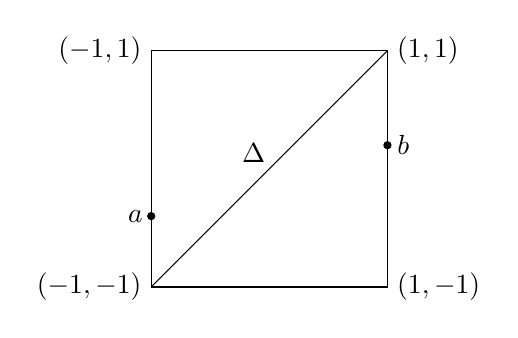
\begin{tikzpicture}
		\draw (-1.5,1.5)node[left]{$(-1,1)$}--(1.5,1.5)node[right]{$(1,1)$}--(1.5,-1.5)node[right]{$(1,-1)$}--(-1.5,-1.5)node[left]{$(-1,-1)$}--(-1.5,1.5);
		\draw (-1.5,-1.5)--(1.5,1.5);
		\node at (-1.7,-.6){$a$};
		\node at (1.7,.3){$b$};
		\fill (-1.5,-.6) circle (1.5pt);
		\fill (1.5,.3) circle (1.5pt);
		\node at (-.2,.2){$\Delta$};
	\end{tikzpicture}
\end{figure}
%\noindent{\heiti 证法2}.我们在正方形$D^1\times D^1$中考虑$f$的图像$G:=\{(x,f(x))\colon x\in D^1\}$,如上图所示.\\
%设$f(-1)=a,f(1)=b$.若$f(-1)=-1$或$f(1)=1$,则命题得证,因此设$a>-1,b<1$.设$\Delta$是恒等映射的图像(即正方形的对角线),则我们只需证$G\cap\Delta\neq\varnothing$.将$G$看作连续映射$x \mapsto(x,f(x))$的像集,则由$f$连续知$G$连通.\\
%定义$A=\{(x,f(x)):f(x)>x\},B=\{(x, f(x)):f(x)<x\}$,则$a\in A,b\in B$,故$A,B$非空.假若$G\cap\Delta=\varnothing$,则按定义有$G$是$A$和$B$的不交并\[G=A\cup B.\]最后,容易验证$A$和$B$都是$G$中开集,这与$G$的连通性矛盾.
遗憾的是,上述证明没有高维的推广(特别地, $n=2$的情形可以用代数拓扑中基本群的工具解决).美国数学家莫里斯-赫希(M.W.Hirsch, 1933-)利用单纯逼近定理给出了一个证明;另有分析学的证明,其主要思想是利用适当的光滑函数来逼近$f$;最常见的(也是最初的)还是代数拓扑的证明.在证明中,我们构造了一个“同调函子”$H_n$将问题进行转化,具体过程这里略去了.

简而言之,代数拓扑的强大工具将本问题转移到了代数领域,并在那里将问题解决.在拓扑学中,这一结果与Jordan曲线定理、毛球定理、维数不变性定理(这一重要结果的论证在1911年也由布劳威尔给出)和Borsuk–Ulam定理一样,是表征欧氏空间拓扑的关键定理之一.

%\begin{enumerate}
%\item 对每个拓扑空间$X$,都存在Abel群$H_n(X)$;
%\item 对每个连续函数$f:X\to Y$,都有同态$H_n(f):H_n(X)\to H_n(Y)$,当$g\circ f$有定义时,满足\begin{equation}H_n(g\circ f)=H_n(g)\circ H_n(f).
%\end{equation}
%\item 若$\id_X$是$X$上的恒等映射,则\begin{equation}
%		H_n(\id_X)\text{~是~}H_n(X)\text{~上的恒等映射};
%\end{equation}
%\item
%\begin{align}
%	&H_n(D^{n+1})=0(n\geq1);\\
%	&H_n(S^n)\neq0(n\geq1).
%\end{align}
%\end{enumerate}
%下面我们利用$H_n$和它的四条性质来证明Brouwer不动点定理.
%\begin{definition}
%拓扑空间$Y$的子空间$X$称为$Y$的\textbf{收缩核},如果存在连续映射$r:Y\to X$满足$r(x)=x,\forall x\in X$.映射$r$称为\textbf{收缩映射}.
%\end{definition}
%\begin{corollary}\label{cor:4}
%设$i:X\hookrightarrow Y$是包含映射,则连续映射$r:Y\to X$是收缩映射当且仅当$r\circ i=\id_X$.
%\end{corollary}
%\begin{lemma}
%若$n\geq0$,则$S^n$不是$D^{n+1}$的收缩核.
%\end{lemma}
%\begin{proof}
%先设$n\geq1$.反证,设有收缩映射$r:D^{n+1}\to S^n$,则下面关于拓扑空间和连续映射的图表应当交换:\begin{center}
%\begin{tikzcd}[column sep=small]
%												&D^{n+1}\arrow[dr,"r"] & \\
%	S^n\arrow[ur,"i"]\arrow{rr}{\id}& 								& S^n
%\end{tikzcd}
%\end{center}
%(这里交换指的是$r\circ i=\id_{S^n}$).将$H_n$作用在此交换图上,得到一个关于交换群和群同态的图表:\begin{center}
%\begin{tikzcd}[column sep=small]
%	&H_n(D^{n+1})\arrow[dr,"H_n(r)"] & \\
%	H_n(S^n)\arrow[ur,"H_n(i)"]\arrow{rr}{H_n(\id)}& & H_n(S^n).
%\end{tikzcd}
%\end{center}由(1)知新图表也应交换: $H_n(r)\circ H_n(i)=H_n(\id)$.又由(3)知$H_n(D^{n+1})=0$,因而$H_n(\id)=0$.但是由(2)知$H_n(\id)$是$H_n(S^n)$上的恒等映射,这与(4)矛盾.\\
%$n=0$的情形是平凡的.事实上,收缩映射显然是满射.因此$r:D^1\to S^0$是从$[-1,1]$到$\{\pm1\}$的连续映射,这是不可能的.
%\end{proof}
%通过此引理,我们可以看到同调函子将拓扑问题转化成了代数问题.我们现在终于可以给出Brouwer不动点定理的证明.
%\begin{proof}
%反证,设$f(x)\neq x,\forall x\in D^n$,因此$x$和$f(x)$两点便确定了一条直线.定义函数$g:D^n\to S^{n-1}$如下(注意$S^{n-1}$是$D^n$的边界):对于$x\in D^n$,设$g(x)$为射线$\overline{f(x)x}$与$S^{n-1}$的交点.显然当$x\in S^{n+1}$时有$g(x)=x$.读者可用解析几何知识验证$g$的连续性,这便与引理1矛盾.
%\end{proof}

\end{document}
